\documentclass[acmsmall,review,nonacm]{acmart}\settopmatter{printfolios=true,printccs=false,printacmref=false}

\AtBeginDocument{%
	\providecommand\BibTeX{{%
			\normalfont B\kern-0.5em{\scshape i\kern-0.25em b}\kern-0.8em\TeX}}}

\setcopyright{acmcopyright}
\copyrightyear{2018}
\acmYear{2018}
\acmDOI{10.1145/1122445.1122456}

\usepackage{listings}
\usepackage{lipsum}
\usepackage{xcolor}
\usepackage{multirow}


%% These commands are for a PROCEEDINGS abstract or paper.
\acmConference[Woodstock '18]{Woodstock '18: ACM Symposium on Neural
	Gaze Detection}{June 03--05, 2018}{Woodstock, NY}
\acmBooktitle{Woodstock '18: ACM Symposium on Neural Gaze Detection,
	June 03--05, 2018, Woodstock, NY}
\acmPrice{15.00}
\acmISBN{978-1-4503-XXXX-X/18/06}


\begin{document}
	
	\title{Fine-grained Reductions Around CFL Reachability}
	
	\author{Aleksandra Istomina}
	\thanks{Aleksandra Istomina: graduate student, email: aleksandra2999@mail.ru, ACM student member number: 4678238}
	\email{aleksandra2999@mail.ru}
	\affiliation{%
		\institution{Saint Petersburg State University}
		\city{Saint Petersburg}
		\country{Russia}
	}
	\affiliation{%
	\institution{JetBrains Research}
	\city{Saint Petersburg}
	\country{Russia}
	}

    \author{Research advisor: Semyon Grigorev}
    \affiliation{%
    	\institution{Saint Petersburg State University}
    	\city{Saint Petersburg}
    	\country{Russia}
    }
    \affiliation{%
    	\institution{JetBrains Research}
    	\city{Saint Petersburg}
    	\country{Russia}
    }
	
	\newcommand\todo[1]{{\color{violet}#1}}
	\newcommand\db[1]{{\color{red}#1}}
	\newcommand\question[1]{{\color{cyan}#1}}


	\maketitle
	
	\section{Introduction}
	
	CFL Reachability problem finds application in different fields of research: static code analysis (e.g. type-based flow analysis~\cite{10.1145/373243.360208} or points-to analysis~\cite{10.1145/1103845.1094817, 10.1145/1133255.1134027}), graph databases, bioinformatics. It finds valid paths between vertices in a graph. 
	
	There are several cubic~\cite{10.1145/298514.298576, 10.1145/199448.199462} and slightly subcubic~\cite{10.1145/1328438.1328460} algorithms for CFL rechabilty. The big open question is whether truly subcubic algorithm exists. 
	
	maybe we can prove that no such algorithm exist under some hypothesis
	
	\subsection{\todo{main problem}}
	
	fine-grained complexity has some results in the area
	
	results are scattered, have no structure
	
	maybe everything is already proven
	
	\subsection{\todo{main goals, overview}}
	
	collect existing results into easy-to-read form
	
	focus on static, dynamic problems are omitted from this research
	
	state open problems
	
	\section{Preliminaries}
	
	\emph{Context-free grammar} (CFG) is a triple $G=(N, \Sigma, R)$, where $N$ is a set of nonterminals, $\Sigma$ is a set of terminals and $R$ is a set of productions of the followings form: $A \to \alpha$, $\alpha \in (N \cup \Sigma)^*$. Denote a context-free language of words derived from the starting symbol $S \in N$ as $L_S(G)$.
	
	\emph{CFG Recognition} problem is to decide whether $w \in L(G)$ given a CFG $G$ and a string $w \in \Sigma^*$. This problem is closely related to \emph{CFG parsing problem} where we want a possible derivation sequence, if $w \in L(G)$. It is known~\cite{10.5555/646233.682379} that CFG recognition is as hard as CFG parsing up to logarithmic factors.
		
	Let $D = (V, E)$ be a directed graph which edges are labelled with symbols from $R$. We call a path from vertex $v$ to vertex $u$ an $S$-path if concatenation of labels on that path is a word from $L_S(G)$.  \emph{Context-free-language (CFL) Reachability} problem~\cite{10.1145/258994.259006} is to determine if there exists an $S$-path between a given sets of vertices $A, B$. In \emph{single source/single target (s-t)} CFL Reachability $A = \{s\}, B = \{t\}, s, t \in V(D)$. In \emph{all-pairs} CFL Reachability $A = B = V(D)$.
	
	\emph{Dyck-$k$} reachability problem is a CFL reachability problem where $G$ defines a Dyck language on $k$ types of parentheses.
	
	For problems $P, Q$ and time bounds $t_P, t_Q$, a \emph{fine-grained reduction}~\cite{bringmann2019fine} from $(P, t_P)$ to $(Q, t_Q)$ is an algorithm that, given an instance $I$ of $P$, computes an instance $J$ of $Q$ such that: 
	
	\begin{itemize}
		\item $I$ is a YES-instance of $P$ if and only if $J$ is a YES-instance of $Q$,
		\item for any $\epsilon > 0$ there is a $\delta > 0$ such that $t_Q(|J|)^{1 - \epsilon} = \mathcal{O}(t_P (|I|)^{1 - \delta})$, 
		\item the running time of the reduction is $\mathcal{O}(t_P (|I|)^{1 - \gamma})$ for some $\gamma > 0$.
	\end{itemize}

	

	
	\section{Main Results}
	
	\begin{figure}[!htp]
		
		\begin{center}  
			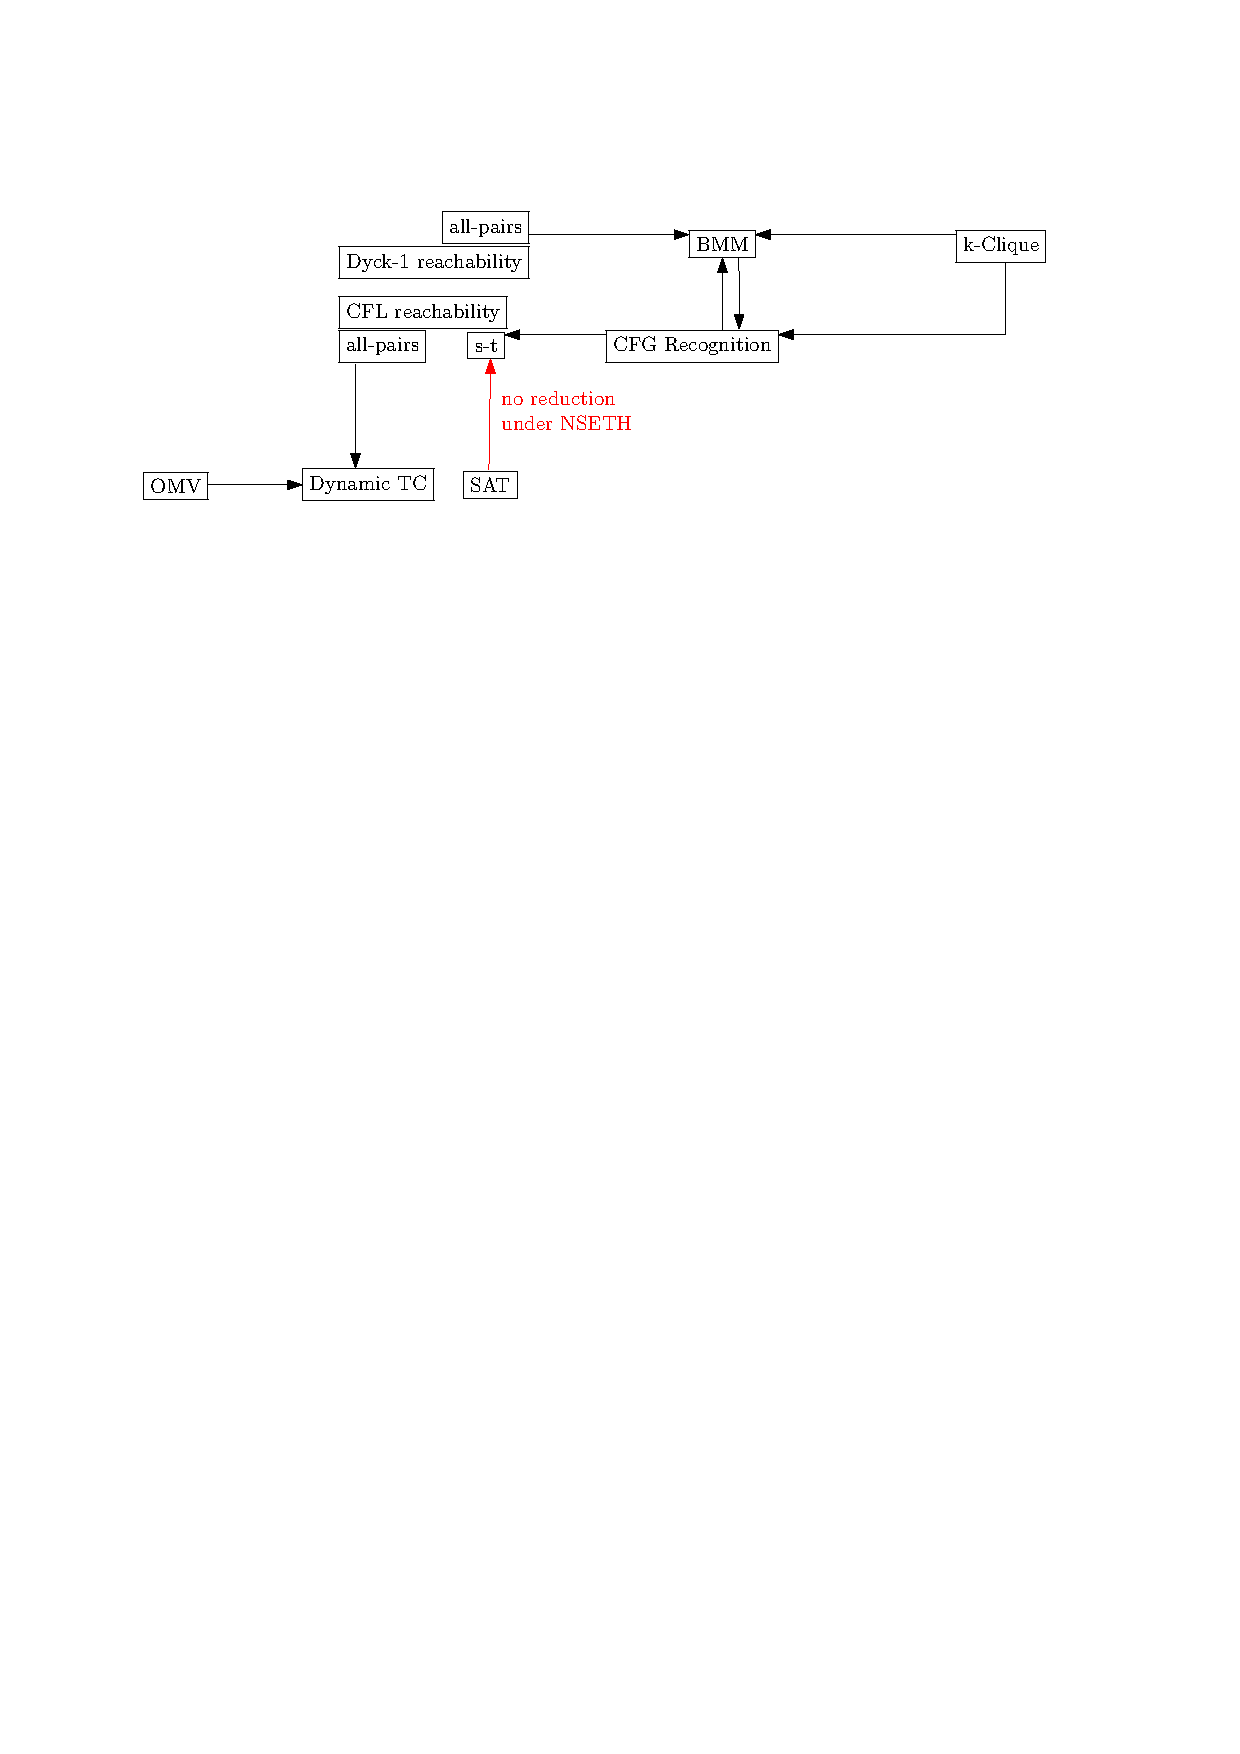
\includegraphics[scale = 0.6]{map_popl.pdf}
		\end{center}
	
		\caption{Black arrow $a \rightarrow b$ represent existing reduction from $a$ to $b$, directions of future work are marked with dashed arrows. Red and turquoise arrows analogously represent non-existence of the reduction and open problems respectively. }
		
	\end{figure}
	
	\subsection{existing problems and hypotheses}
	
	There are several problems that are connected with CFL Recognition and Reachability. 
	
	\emph{Boolean satisfiability problem (SAT, $k$-SAT)} is to determine if there exists an interpretation of variables that satisfies a given Boolean formula on $n$ variables written in $k$-CNF, $k > 3$. The hypothesis about SAT, that we are interested about, is NSETH~\cite{10.1145/2840728.2840746} which proposes that there is no $\epsilon > 0$ such that $k$-SAT can be solved co-nondeterministically in time $2^{(1 - \epsilon) n}$ for any $k$.
	
	In \emph{Boolean Matrix Multiplication (BMM)} problem it is needed to calculate matrix product of the two given $n \times n$ matrices over (AND, OR). BMM hypothesis states that there is no $\mathcal{O}(n^{3 - \epsilon})$ combinatorial algorithm for that. 
	
	\emph{Orthogonal Vectors (OV)} problem decides whether two sets $X, Y$ of $n$ boolean $d$-dimensional vectors contain a pair $x \in X, y \in Y$ which dot product $x \cdot y$ equals zero. Hypothesis states that OV problem can not be solved in $\mathcal{O}(n^{2 - \epsilon} \cdot poly(d))$ time. 
	
	Given a context free language $L(G)$ the \emph{Language Edit Distance (LED)} problem seeks the minimum number of edits (insertions, deletions and substitutions) required to convert the given string $s$ into a member of $L(G)$. 
	
	The incremental \emph{dynamic transitive closure (DTC)}~\cite{Hanauer2020FasterFD} problem asks to maintain reachability information in a directed graph between arbitrary pairs of vertices under insertions of edges.
	
	\subsection{\todo{existing reductions}}
	
	CLFLR <-> SetConstr
	
	The problem has been shown to be 2NPDA-hard~\cite{10.5555/788019.788876},which yields a conditional cubic lower bound in its complexity.
		
	dynamic TC to all-pairs
	
	BMM to Dyck-1
	
	s-t -> cfg -> bmm => no combinatorial algorithm
	
	short s-t certificates => no reduction from SAT
		
	\subsection{open problems}
	
	This paper is a part of research dedicated to determination of existence or non-existence of a truly subcubic algorithm for CFL Reachability. Apart from that there area several open problems in the are worth mentioning. 
	
	It is known~\cite{10.1145/3186893} that detecting one triangle of a total negative edge weight in a weighted graph and up to $n^{3 - \epsilon}, \epsilon > 0$ such triangles are subcubic equivalent tasks. Analogous question arises for s-t and all-pairs CFL reachability.
	
	 There exists a reduction from Andersen pointer analysis~\cite{10.1145/3434315} to OV problem where as a part of reduction appears slightly modified Dyck-1 reachability with additional if-condition for edge existence in a graph. The question is if similar reduction exists to pure Dyck-1 problem. Existence of such a reduction would provide a conditional quadratic lower bound on Dyck-1 reachability problem, now there is no non-trivial one.
	 
	 All-pairs shortest paths (APSP) problem and it's subcubic equivalent analogues~\cite{10.1145/3186893} is connected to problems on paths. Finding a fine-grained reduction from APSP to CFL reachability would give a conditional lower bound on a complexity of a problem.
	
	\section{Conclusion and Future work}
	
	CFL reachability is a popular problem strongly connected with many areas. It has several cubic algorithms and no truly subcubic combinatorial one under BMM hypothesis. It has been proved that we can't get cubic lower bound on CFL reachability using reduction from SAT under NSETH. 
	
	Still other reductions may be possible. For example, OMV problem is connected to dynamic problems as is CFL reachability and APSP to problems on paths. Getting cubic lower bound through them is a possible way of future work. 
	
	This overview was focused on static problems and reductions between them. There is a big field of dynamic problems where are many reductions of our interest. We plan to extend our research there. 
	
	\section{Acknowledgments}
	
	\bibliographystyle{ACM-Reference-Format}
	\bibliography{map}
	
	\appendix
	
\end{document}
\endinput
